\newpage
\section{Durchführung}
\label{sec:Durchführung}

\subsection{Justage der Laserdiode}
\label{sec:Justage}

Zunächst wurde die Laserdiode auf dem optischen Tisch positioniert und
bei niedrigstem Strom eingeschaltet. Die Temperatur wurde dauerhaft auf \SI{50}{\celsius} geregelt.
Unter Verwendung einer Infrarot (IR) Detektionskarte lässt sich der Laserstrahl sichtbar machen.
Dafür wird nun der Injektionsstrom erhöht, bis ein Lichtpunkt auf der Karte sichtbar ist.
Der eingestellte Injektionsstrom wird mit Hilfe eines Amperemeters gemessen.
Für ein besseres Bild nimmt eine CCD Kamera den Lichtpunkt auf der Karte auf und
zeigt diesen auf einem Bildschirm an.
Mit Hilfe dieses in Abbildung \ref{fig:ExternalCavityAlignment} dargestellten Aufbaus
lässt sich der externe Resonator der Laserdiode justieren.

\begin{figure}
	\centering
	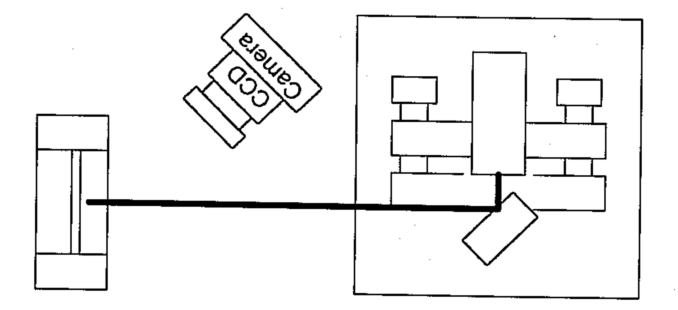
\includegraphics[width=.6\textwidth, angle=1, origin=c]{images/ExternalCavityAlignment.pdf}
	\caption{Justage des externen Resonators \cite{anleitung}.}
	\label{fig:ExternalCavityAlignment}
\end{figure}

Der Injektionsstrom wird so eingestellt, dass die Verstärkung durch induzierte
Emission gerade etwas höher ist als optische Verluste.
Auf der IR Karte zeigt sich das Lasen durch eine Auffächerung des hellen Punktes in ein
Interferenzmuster des Gitters, das als äußerer Resonator fungiert.
Diese Auffächerung ist in Abbildung \ref{fig:laser-pattern} dargestellt.

\begin{figure}
	\centering
	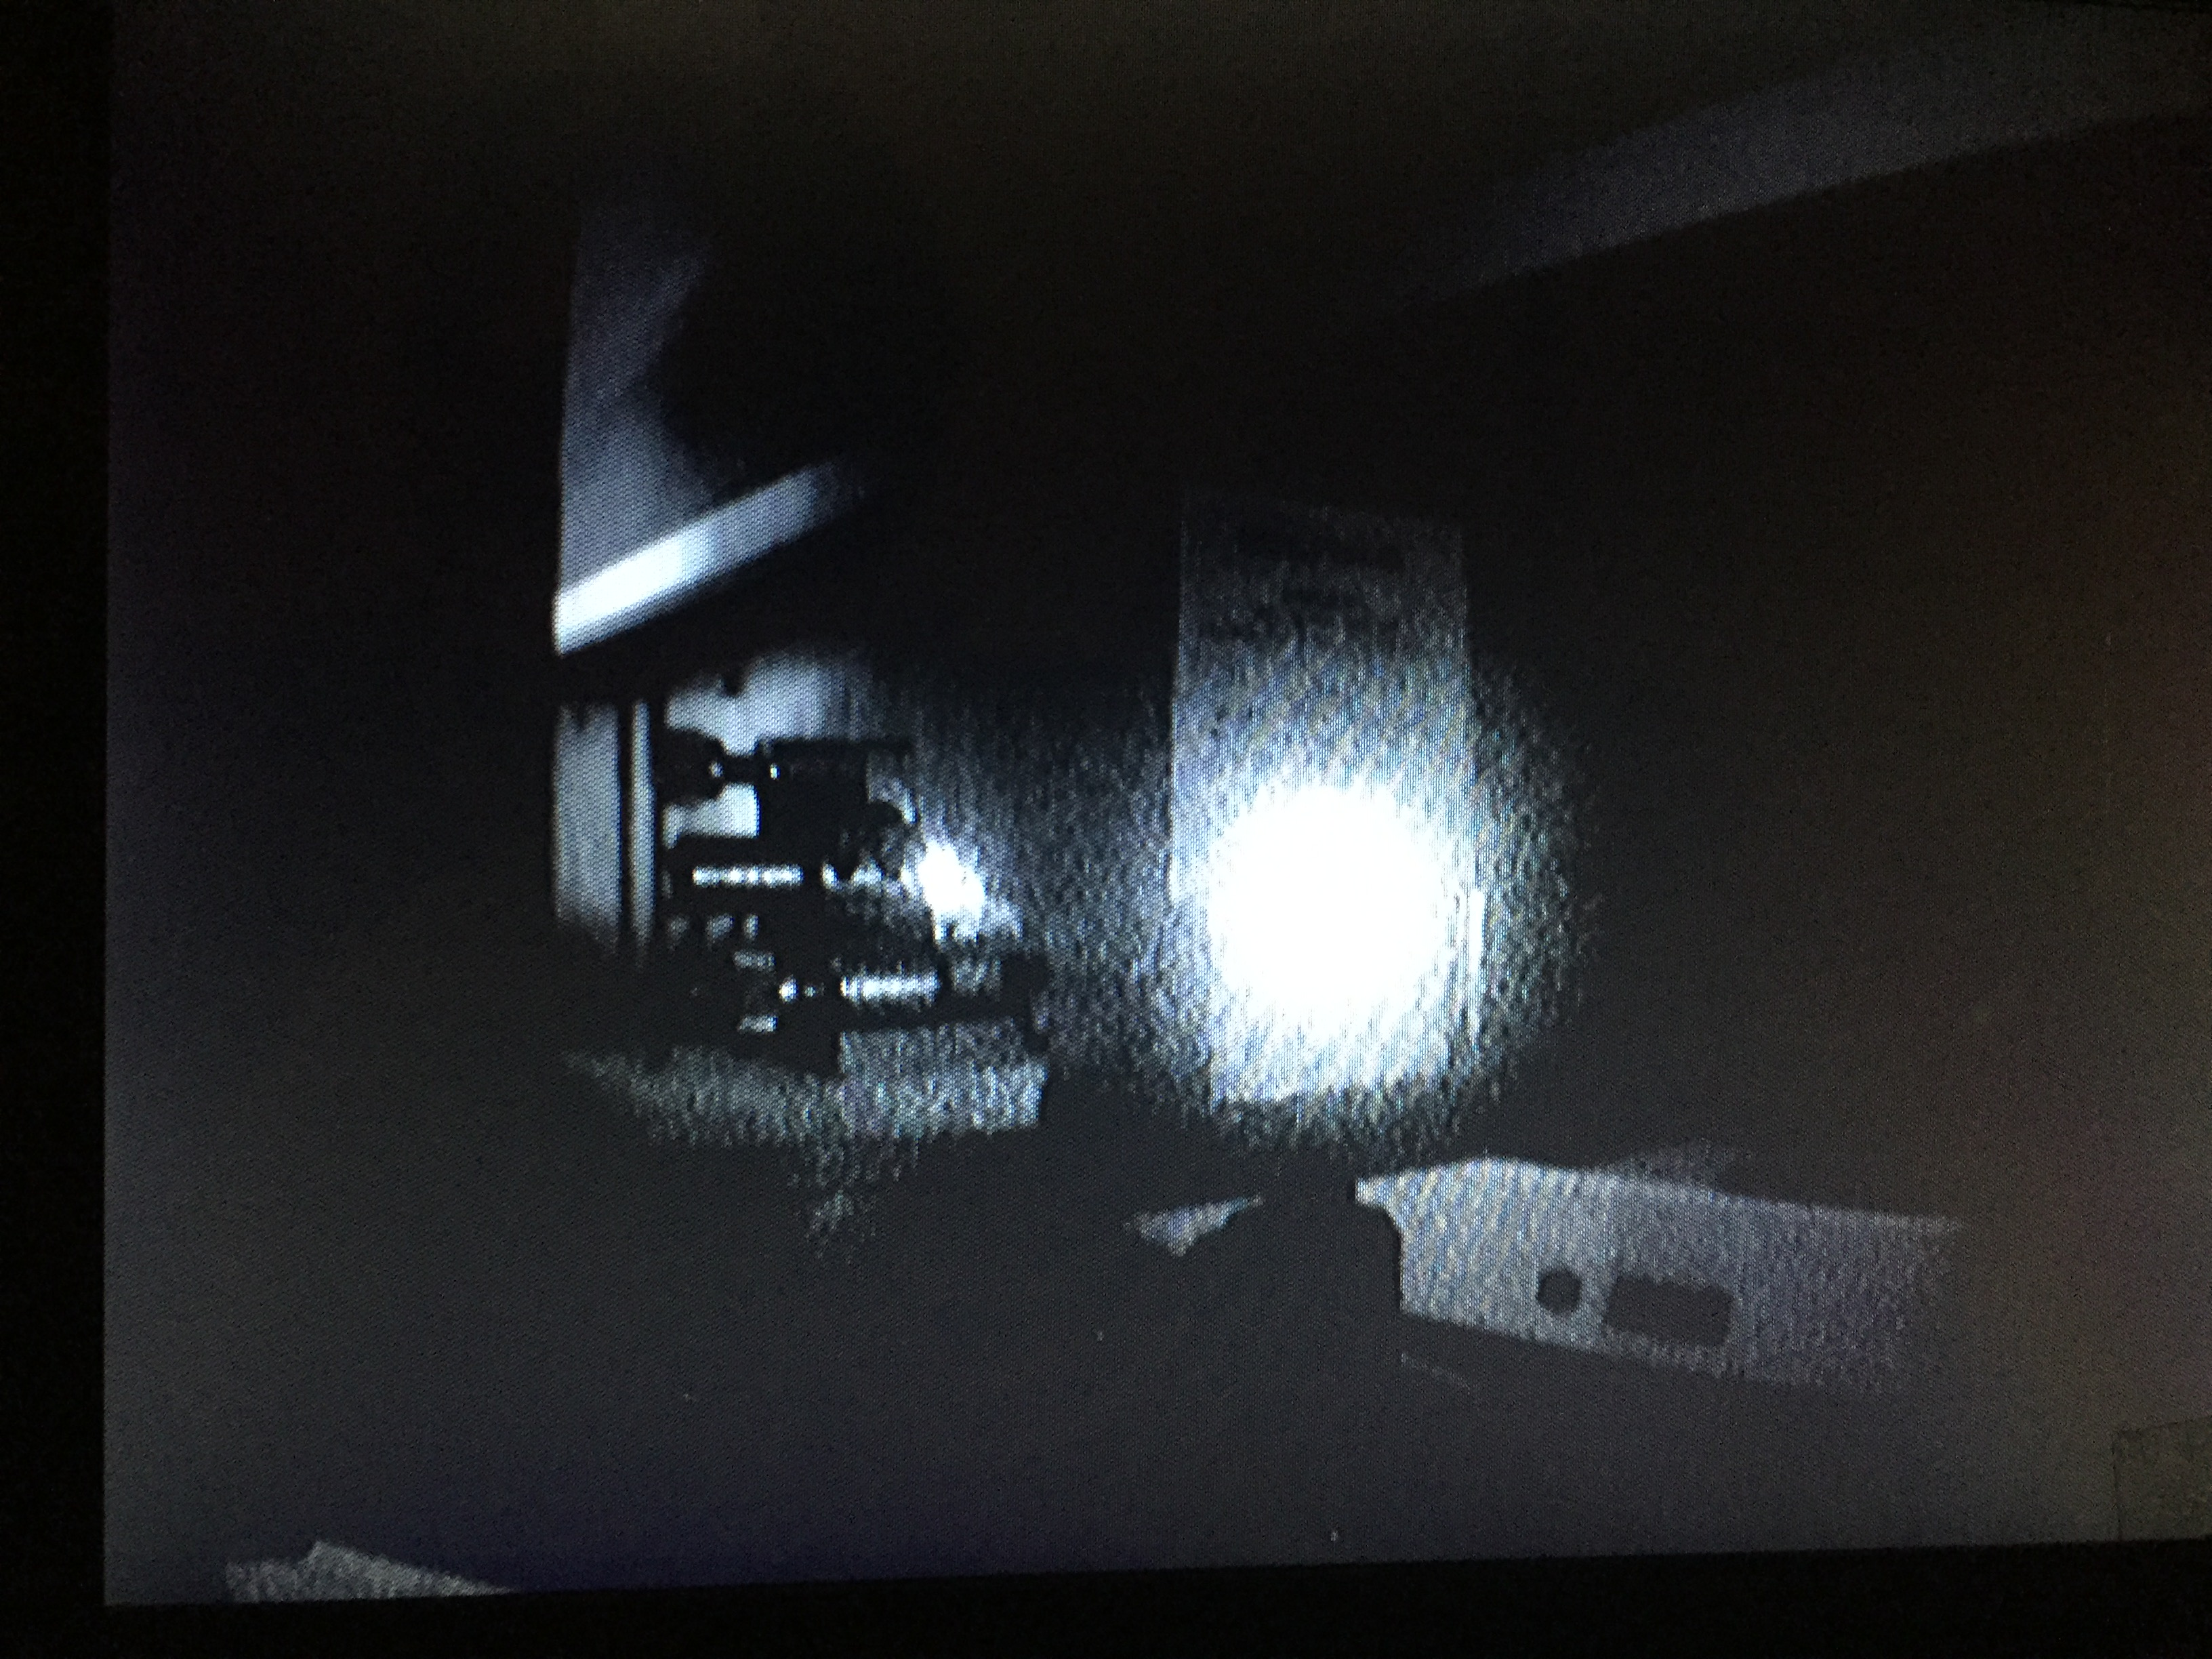
\includegraphics[width=.5\textwidth]{images/laser-pattern.JPG}
	\caption{Auffächerung des Laserpunktes auf der IR Karte.}
	\label{fig:laser-pattern}
\end{figure}

Mit Hilfe des TOP-Drehknopfes der Laserdiode lässt sich der Winkel des Gitters und
dessen Abstand zum Dioden-Chip einstellen.
Wird dieser verändert, lassen sich mit dem Auge mehrere Intensitätsmaxima beobachten.
Der Drehknopf wird auf eines dieser Maxima ungefähr in der Mitte der Serie eingestellt.
Im Anschluss lässt sich die Intensität des Injektionsstroms ein wenig herunter regeln,
bis der Laser knapp unter dem Schwellwert zum Lasen ist.
Mit erneuter Justage des TOP-Drehknopfes lässt sich das Lasen der Diode wiederherstellen.
Diese Prozedur wird solange wiederholt, bis eine untere Grenze erreicht ist und der
Strom nicht weiter herunter geregelt werden kann, ohne dauerhaft unterhalb des
Schwellwerts zu bleiben.


\subsection{Aufnahme des Fluoreszenzspektrums von Rubidium}
\label{sec:Rb-Fluoreszenz}

Für die Beobachtung des Fluoreszenzspektrums von Rubidium ist der Versuchsaufbau
wie in Abbildung \ref{fig:RbFlorescenceSetup} dargestellt anzupassen.
Der Lasterstrahl läuft durch die Rubidiumprobe und trifft auf die IR Karte,
um mögliche Reflexionen im Raum zu vermeiden.
Seitlich an der Apperatur befindet sich eine Bohrung, durch welche das
Fluoreszenzlicht tritt und von der CCD Kamera erfasst wird.

\begin{figure}
	\centering
	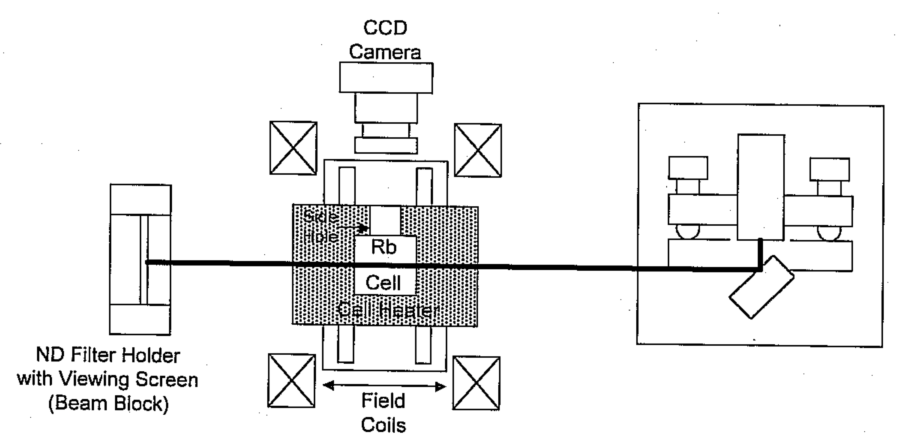
\includegraphics[width=.8\textwidth, angle=1, origin=c]{images/RbFlorescenceSetup.pdf}
	\caption{Schematischer Aufbau zur Beobachtung der Rubidium Fluoreszenz \cite{anleitung}.}
	\label{fig:RbFlorescenceSetup}
\end{figure}

Um Fluoreszenzlicht beobachten zu können, wird der Injektionsstrom etwas über den
bisher eingestellten Grenzstrom eingestellt.
Nun wird das Gitter des externen Resonators horizontal mit dem SIDE Drehknopf
verschoben, bis auf dem Bildschirm der CCD Kamera ein heller Streifen sichtbar ist,
wo Photonen des Laserlichts vom Rubidium absorbiert werden.
Dieser helle Streifen ist in Abbildung \ref{fig:RbFlorescence} dargestellt.

\begin{figure}
	\centering
	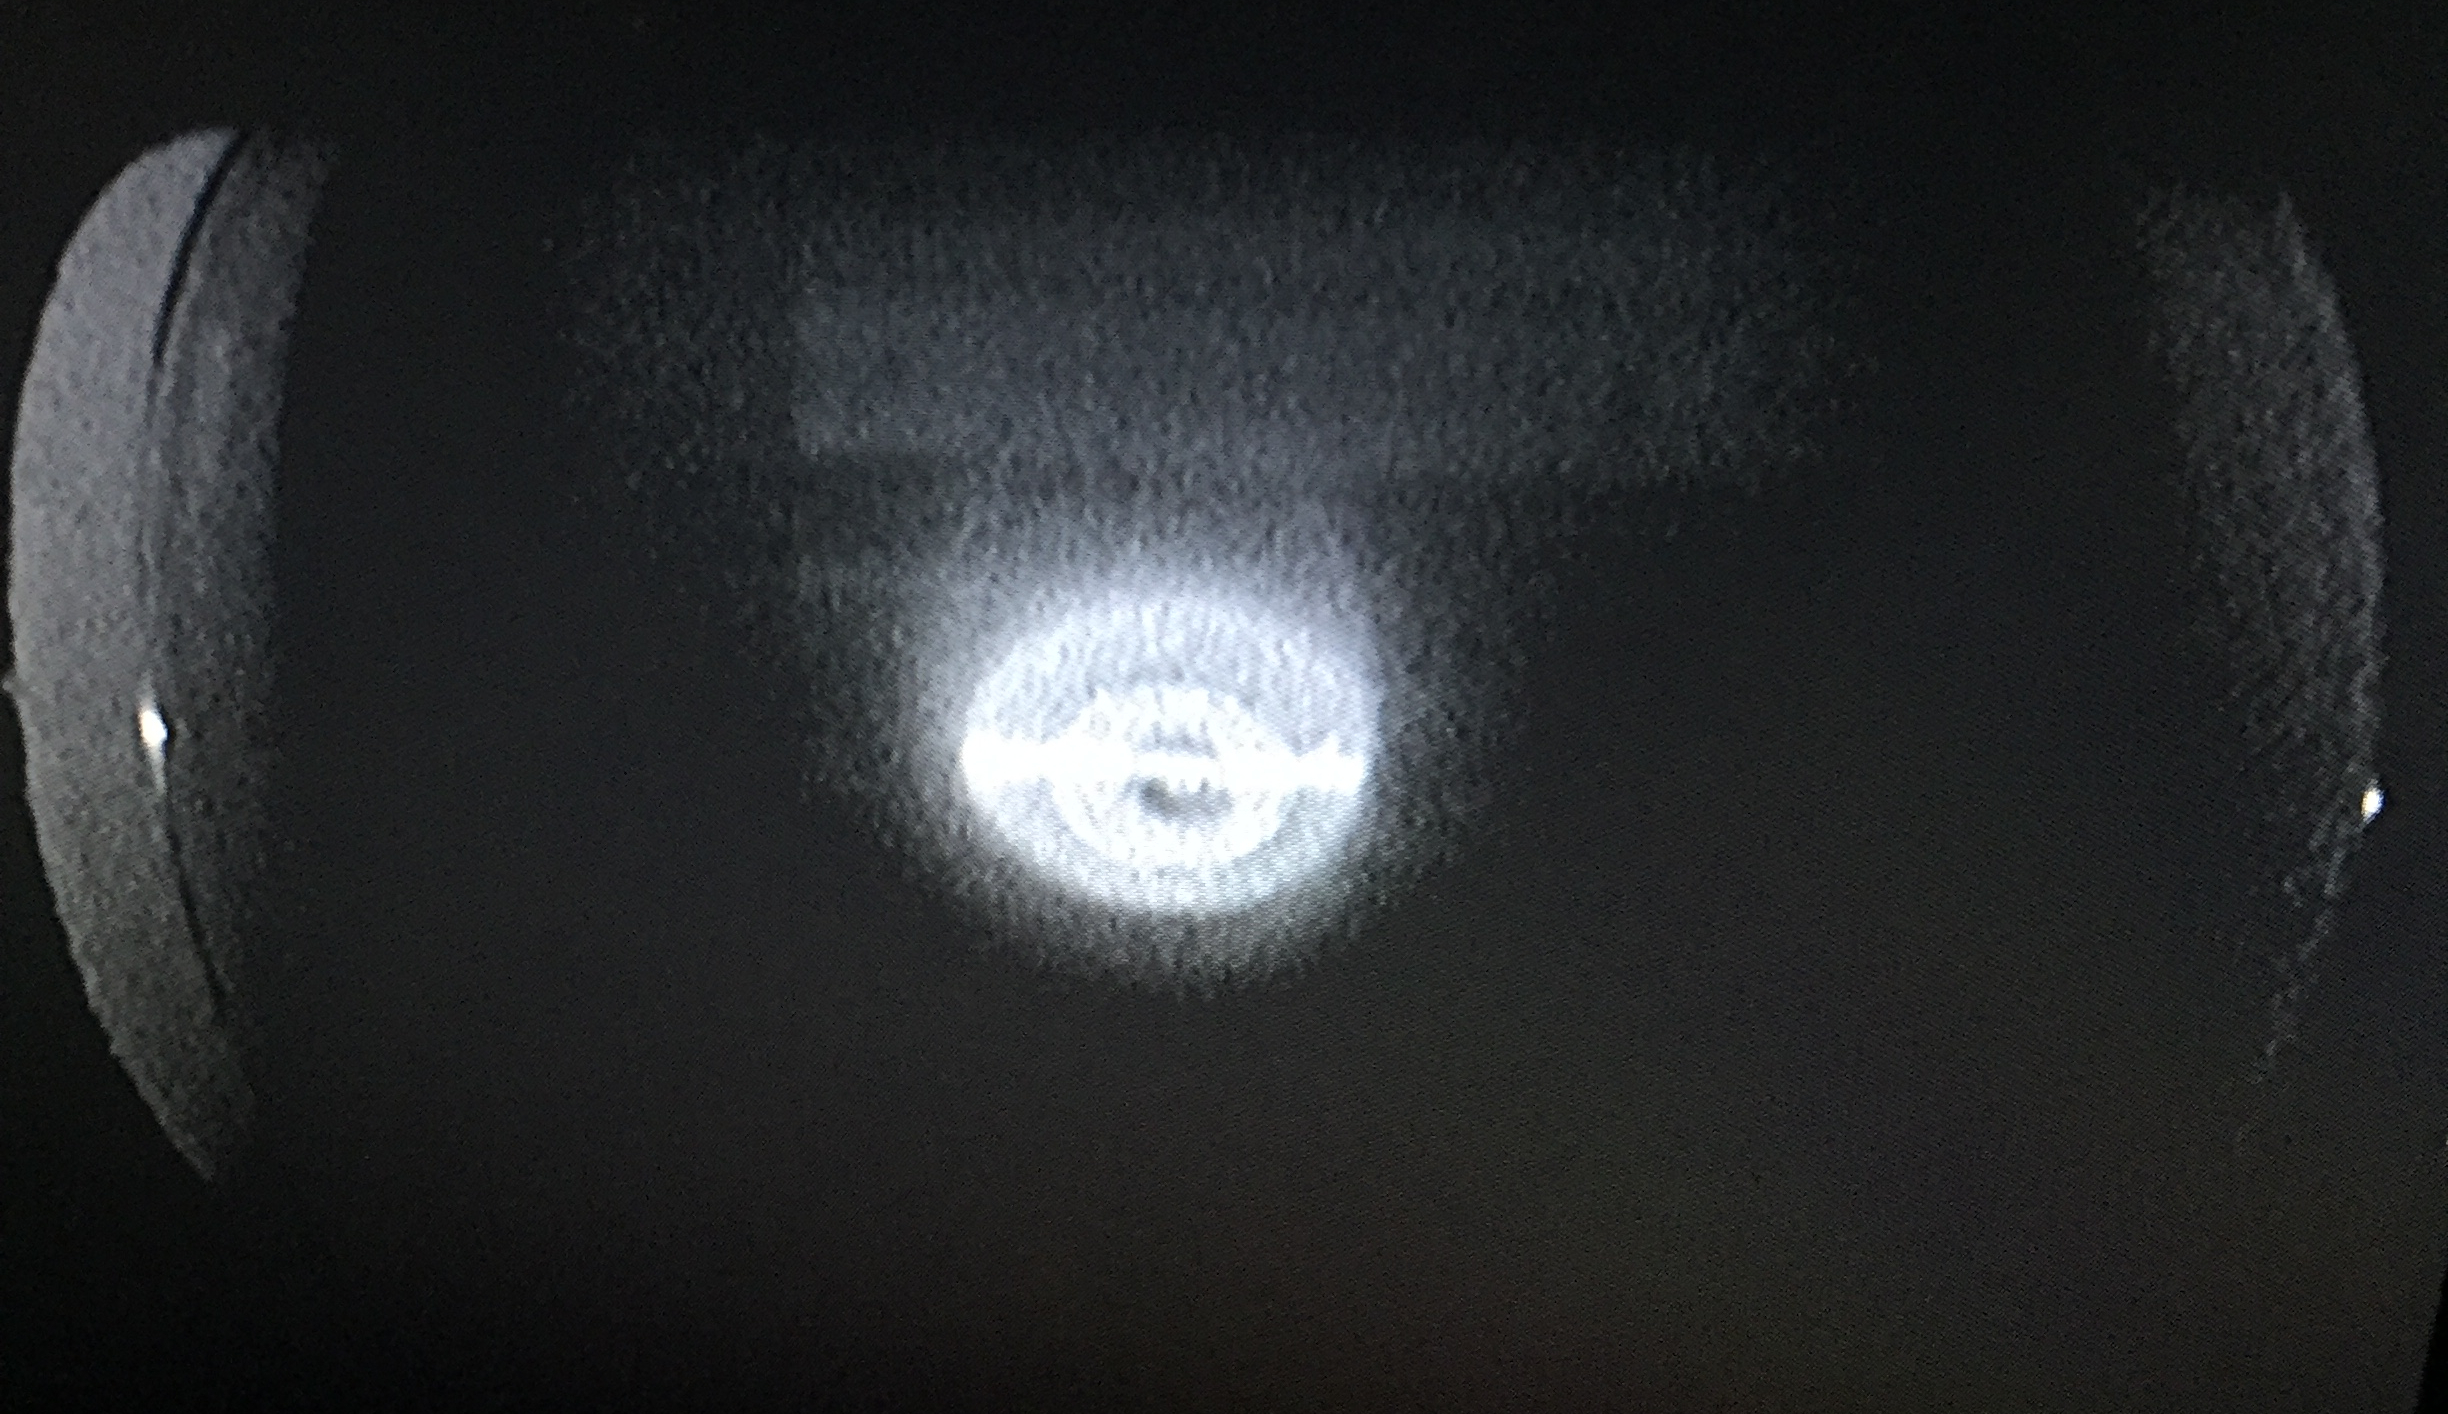
\includegraphics[width=.6\textwidth]{images/florescence.JPG}
	\caption{Mit der CCD-Kamera aufgenommenes Bild der Rubidium Fluoreszenz.}
	\label{fig:RbFlorescence}
\end{figure}

Im Anschluss wird ein RAMP Generator mit einer Frequenz von \SI{10}{\hertz} verwendet,
um das Gitter zu verschieben. Dazu wird der Generator an einen Piezo Kristall
angeschlossen, welcher die Position des Gitters steuert. Weiterhin wird
das Signal des Generators auf einem Oszilloskop angezeigt.
Zusätzlich wird die IR Karte hinter der Rubidiumprobe durch eine Photodiode (PD)
ersetzt, welche ebenfalls an das Oszilloskop angeschlossen wird.
Um zu verhindern, dass die PD durch das Laserlicht gesättigt wird, wird
in den Strahlengang zwischen Laserdiode und Probe ein Neutraldichtefilter plaziert.
Nun wird die Empfindlichkeit der Photodiode auf die maximale Empfindlichkeit
eingestellt, ohne zu saturieren.

\begin{figure}
	\centering
	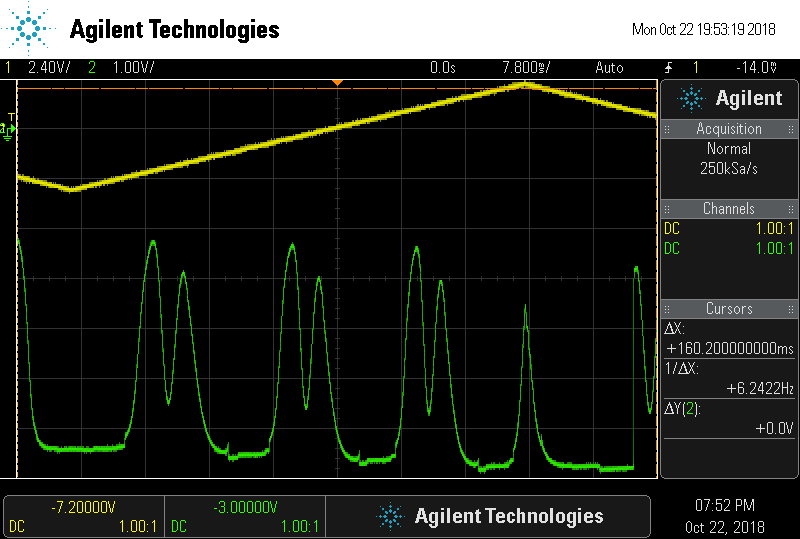
\includegraphics[width=.8\textwidth]{images/first-signal.png}
	\caption{Bildschirmaufnahme des Oszilloskops, welches das Sägezahnsignal des
	RAMP Generators und zwei Absorptionsdips aufgrund des Rubidiumdampfes zeigt.}
	\label{fig:first-signal}
\end{figure}

In Abbildung \ref{fig:first-signal} ist das erhaltene Bild des Oszilloskops dargestellt.
Getriggert wurde auf die aufsteigende Flanke des RAMP Generators, welcher als gelbe
Kurve dargestellt ist. In grün ist das Signal der Photodiode dargestellt, welches
im Laufe der Zeit verschiedene Peaks zeigt. Diese Peaks sind (unter Berücksichtigung
der Ausrichtung der y-Achse nach unten) die Absorptionsdips des
Laserlichts aufgrund von Anregung von Zuständen des Rubidiumdampfes.
Kleine Zacken im Signal zeigen an, dass es im Laufe eines Durchlaufs des Generators
zu verschiedenen Modensprüngen kommt, sodass die selben Absorptionsdips mehrfach
dargestellt sind.
Durch Variation des Gitter mit Hilfe des SIDE Drehknopfes lassen sich verschiedene
Moden durchfahren. Leider war es bei der Durchführung des Versuchs nicht möglich,
andere Moden als die zwei in Abbildung \ref{fig:first-signal} dargestellten zu
beobachten.

\subsection{Aufnahme der ersten vier Absorptionslinien von Rubidium}
\label{sec:AbsorptionImproved}

Um mehr als zwei Absorptionsdips ohne Modensprünge beobachten zu können, werden im Folgenden
sowohl das Gitter mit Hilfe eines Piezo Kristalls, als auch der Injektionsstrom
mit Hilfe des RAMP Generators variiert.
Der Aufbau wird soweit verändert, dass das Signal des RAMP Generators nun ebenfalls
in den CURRENT MODULATION INPUT gespeist wird.
Es ergibt sich das in Abbildung \ref{fig:second-signal} dargestellte Bild des
Oszilloskops.

\begin{figure}
	\centering
	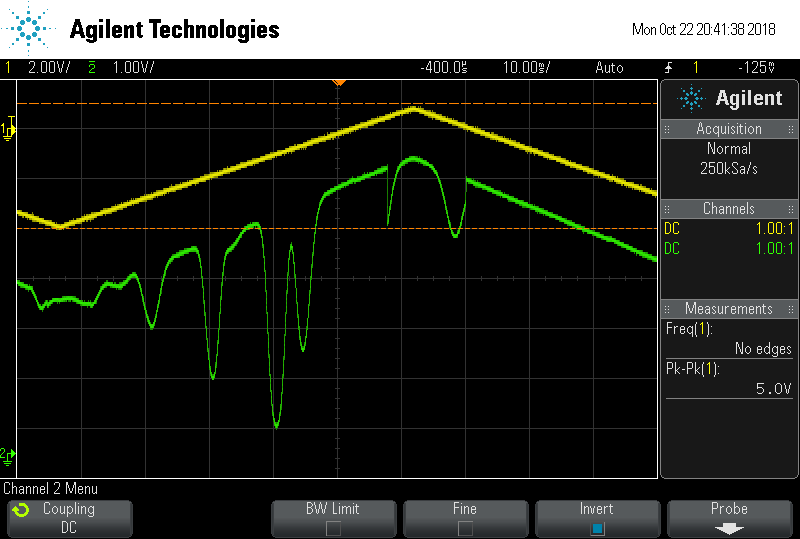
\includegraphics[width=.8\textwidth]{images/second-signal.png}
	\caption{Bildschirmaufnahme des Oszilloskops, welches das Sägezahnsignal des
	RAMP Generators und vier Absorptionsdips aufgrund des Rubidiumdampfes zeigt.}
	\label{fig:second-signal}
\end{figure}

Aufgrund der variierten Laserintensität (über den Injektionsstrom) verändert sich
die Hintergrundintensität des Absorptionssignals, sodass die grüne Linie nach
links oben zu laufen scheint. Dieser Effekt kann behoben werden, indem eine
Strahlteiler zwischen den ND Filter und die Rubidiumprobe plaziert wird und
ein zweiter Strahlteil auf eine zweite Photodiode trifft. Dieser Aufbau
ist in Abbildung \ref{fig:SetupImproved} dargestellt.

\begin{figure}
	\centering
	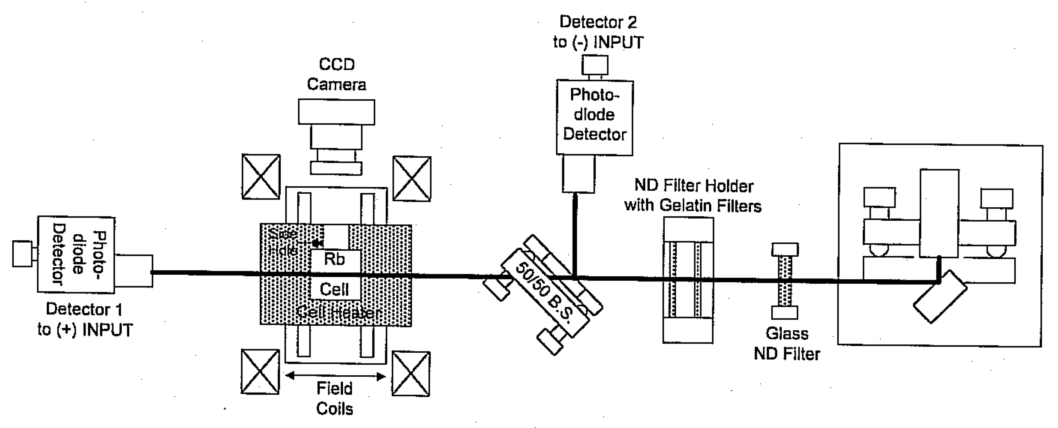
\includegraphics[width=\textwidth, angle=1, origin=c]{images/SetupImproved.pdf}
	\caption{Schematische Skizze des angepassten Versuchaufbaus,
	um Hintergrundintensität mit ein zu beziehen \cite{anleitung}.}
	\label{fig:SetupImproved}
\end{figure}

Beide Photodioden können gegeneinander balanciert werden.
Während der Input der PD hinter der
Rubidiumprobe auf maximaler Balance eingestellt wird, wird die
Balance der zweiten PD langsam erhöht, bis der Effekt der Hintergrundintensität
aufgehoben ist.
Es ergibt sich abschließend das in Abbildung \ref{fig:final-signal} dargestellte
Bild des Oszilloskops.

\begin{figure}
	\centering
	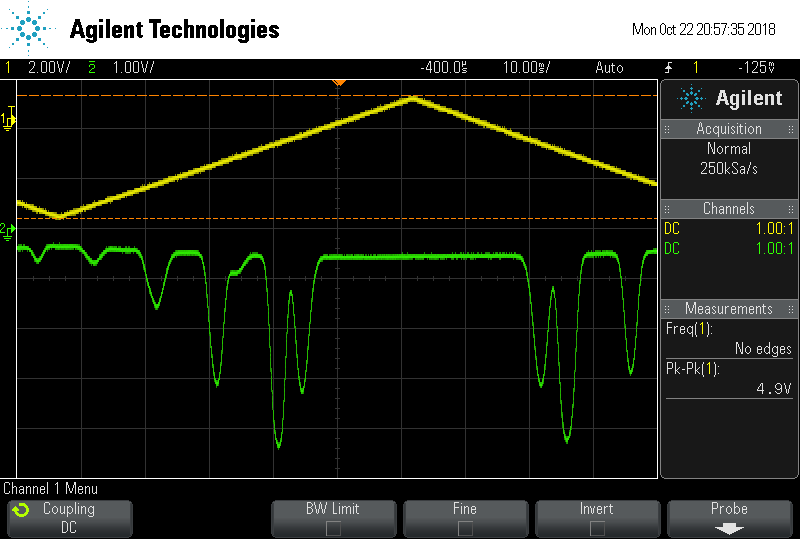
\includegraphics[width=.8\textwidth]{images/final-signal.png}
	\caption{Bildschirmaufnahme des Oszilloskops, welches das Sägezahnsignal des
	RAMP Generators und vier Absorptionsdips aufgrund des Rubidiumdampfes zeigt.
	Die variierende Untergrund wurde dabei abgezogen.}
	\label{fig:final-signal}
\end{figure}
